\documentclass{report}
\setlength{\parindent}{0pt} % Sets the automatic indent size
\usepackage{graphicx} % Required for inserting images
\usepackage{pictex}   % Ensure PicTeX is available
\usepackage{pgfplots}
\usepackage{filecontents}
\usepackage{amsmath}
\usepackage{amssymb}
\usepackage{listings}
\usepackage{xcolor}
\usepackage{float}


\lstset{
    language=C++,
    basicstyle=\ttfamily\tiny,
    keywordstyle=\color{blue}\bfseries,
    commentstyle=\color{gray}\itshape,
    stringstyle=\color{red},
    numbers=none,
    numberstyle=\tiny,
    stepnumber=1,
    breaklines=true,
    frame=single,
    captionpos=b,
    showstringspaces=false
}

\title{HW\#3}
\author{
Elhaam Bhuiyan,
Amir Samarxhiu,
Shaqib Syed
}
\date{\today}

\begin{document}

\maketitle

\section*{Introduction}
Monte Carlo simulation is a fundamental technique for pricing derivatives and estimating expectations under stochastic processes. However, standard Monte Carlo methods can be computationally expensive and exhibit high variance, requiring a large number of simulations to achieve a given level of accuracy. To mitigate this issue, we can use variance reduction techniques to reduce estimator variability without introducing bias. This report explores the implementation of two variable reduction techniques, control variables and antithetic variables, for simulating stock price paths and pricing options. \\

We first establish a baseline by simulating a stock price path using geometric Brownian motion and verify expected values using theoretical properties. Then, we use variance reduction through antithetic variables, a technique that introduces a negatively correlated statistic to stabilize our estimator. We then extend this technique to pricing a European call option. In doing this, we explore the mathematics of pricing a European call option, analyzing how different time steps can affect its valuation. \\

To validate our simulation results, we compare our option price estimates to the closed-form Black-Scholes solution. We then attempt variance reduction through control variables, which uses auxiliary variables with zero expectation to refine our estimator. We explore two different control variables, where each has a different impact on variance reduction and convergence speed. \\

In addition to standard European options, we also price more complex derivatives such as the look-back option, whose payoff is dependent on the maximum stock price during its path. We also explore the shout option, whose payoff can either be fixed at a certain time $\tau < T$, or exercised at expiration. We use the variance reduction techniques described earlier to price each of these, and then compare these option types to each other and to the European option. \\

By analyzing the impact of each variance reduction technique, this report demonstrates the practical impact of variance reduction in financial simulations. Our findings demonstrate to what extent these techniques improve our simulations, emphasizing the necessity of these techniques for accurate and efficient Monte Carlo pricing.

\newpage

\section*{Results}
\subsection*{Problem 1:}
After running the simulation in \texttt{StockPrice.cpp}, we obtained an estimate of the expected discounted stock price, $\overline{V} = 99.9961$, after 70,800,000 simulations. This result closely aligns with the initial stock price $S_0$, which is expected under the risk-neutral pricing framework. The risk-neutral pricing framework ensures that:
\[
e^{-rT} \mathbb{E}[S_T]=S_0
\]
This agreement between the expected discounted stock price and the initial stock price is a direct consequence of choosing the drift term $\mu = r - \frac{\sigma^2}{2}$. This specific value of $\mu$ ensures that the stock price follows a geometric Brownian motion and maintains the fundamental risk-neutral pricing property. \\

To determine the time required to achieve a desired level of accuracy, we estimate the completion time $t^*$. From the Central Limit Theorem, the standard error of the sample mean $\overline{V}$ is:
\[
\hat{\text{Std}}(\overline{V})=\frac{\hat{\text{Std}}(V)}{\sqrt{n}}
\]
To ensure a confidence level of 95\%, the error bound is given by:
\[
1.96 \times \frac{\hat{\text{Std}}(V)}{\sqrt{n}} \leq \epsilon
\]
Since the error rate scales as $\frac{1}{\sqrt{n}}$, reducing the error rate by a factor of $k$ requires $k^2$ more simulations. That means that if our current error estimate is $\hat{\epsilon}$ and it required $n$ simulations, to reduce our error rate to $\epsilon$ would require:
\[
n^* = n \times k^2 = n\times \left(\frac{\hat{\epsilon}}{\epsilon}\right)^2
\]

Because each simulation requires the same amount of computational time, increasing the number of simulations by a factor of $k^2$ also increases the runtime by a factor of $k^2$. This means that if it takes $t$ seconds to reach the current estimated error $\hat{\epsilon}$, then to reach the target error $\epsilon$, the estimated total completion time is:
\[
t^* = t \times k^2 = t\times \left(\frac{\hat{\epsilon}}{\epsilon}\right)^2
\]
\newpage
Below are selected results from the simulation's output. To maintain readability, we present a subset of key values in tables for each problem, while the full output is provided in the Appendix for reference.

\begin{table}[H]
    \centering
    \caption{Convergence of $\overline{V}$ and Estimated Completion Time $t^*$}
    \label{tab:simulation_results}
    \begin{tabular}{rcccc}
        \hline
        $n$ & $\overline{V}$ & Error $\pm$ & $t$ (s) & $t^*$ (s) \\
        \hline
        100000   & 100.0451 & 0.132800 & 0.184   & 129.524 \\
        1000000  & 99.9936  & 0.042046 & 1.791   & 126.677 \\
        5000000  & 99.9943  & 0.018804 & 8.909   & 126.006 \\
        10000000 & 99.9979  & 0.013296 & 17.941  & 126.858 \\
        20000000 & 99.9993  & 0.009403 & 36.026  & 127.412 \\
        50000000 & 99.9957  & 0.005946 & 89.966  & 127.245 \\
        70000000 & 99.9962  & 0.005025 & 126.033 & 127.317 \\
        70800000 & 99.9961  & 0.004997 & 127.483 & 127.326 \\
        \hline
    \end{tabular}
\end{table}


\newpage

\subsection*{Problem 2:}
The simulation in Problem 1 suffered from high runtime due to an excessive number of trials required to achieve sufficient accuracy. To address this, we will implement the antithetic variable method, which reduces variance and accelerates convergence. \\

Antithetic variance reduction works by generating pairs of random variables of the same distribution that are negatively correlated. By averaging these pairs of random variables, we construct a new estimator that retains the same expected value as the original, but with reduced variance. The degree of reduction in variance depends on the strength of the negative correlation. By lowering the variance, this approach accelerates convergence, allowing us to achieve our desired accuracy with fewer samples. \\

To apply antithetic variance reduction to this problem, we note that the process $\widetilde{B}_{t_{i}} = -B_{t_{i}}$ has the same distribution as $B_{t_i}$, but is negatively correlated. By generating a second antithetic path alongside each simulation, we can average both paths to obtain a more stable estimator. Using the geometric Brownian motion model, the stock prices at time $T$ are computed as follows:

\begin{align*}
S_T=S_0\exp((r-\frac{1}{2}\sigma^2)T + \sigma B_T) \\
\widetilde{S}_T=S_0\exp((r-\frac{1}{2}\sigma^2)T + \sigma \widetilde{B}_T)
\end{align*}
Instead of estimating the expected present value of the stock price using only $S_T$ directly, we can use the antithetic estimator:
\[
V = e^{-rT} \times \frac{S_T + \widetilde{S}_T}{2}
\]

Since $S_T$ and $\widetilde{S}_T$ are negatively correlated, their sum has lower variance than either variable individually, reducing the number of simulations required to achieve our desired level of accuracy. \\

Beyond implementing antithetic variance reduction, we can optimize the simulation by accumulating only the Brownian motion increments within the loop. Since Brownian motion has independent increments, the final value $B_T$ is obtained by summing these increments. Given that the stock price follows a geometric Brownian motion, we can recognize that only $B_T$ is needed to compute $S_T$. As a result, we can avoid recomputing $S_t$ at each time step and we can efficiently compute $S_T$ once at the end of the loop, reducing computational cost while obtaining the same result. \\

These optimizations yielded a substantial improvement in runtime. The original simulation required approximately 100 seconds to reach the desired accuracy, whereas the optimized version with variance reduction completed in just 2 seconds. This improved convergence rate allows us to achieve the same level of precision with significant fewer samples, illustrating how effective variance reduction techniques can be.  \\

Below is the output for our simulation:

\begin{table}[H]
    \centering
    \caption{Convergence of $\overline{V}$ and Estimated Completion Time $t^*$}
    \label{tab:simulation_results}
    \begin{tabular}{rcccc}
        \hline
        $n$ & $\overline{V}$ & Error $\pm$ & $t$ (s) & $t^*$ (s) \\
        \hline
        100000  & 99.9930  & 0.019600 & 0.139 & 2.141 \\
        400000  & 100.0007 & 0.009862 & 0.538 & 2.095 \\
        700000  & 99.9996  & 0.007448 & 0.925 & 2.053 \\
        1000000 & 99.9995  & 0.006231 & 1.315 & 2.041 \\
        1300000 & 99.9998  & 0.005468 & 1.700 & 2.033 \\
        1600000 & 99.9977  & 0.004927 & 2.085 & 2.025 \\
        \hline
    \end{tabular}
\end{table}



\newpage
\subsection*{Problem 3:}
To estimate the value of a European call option struck at $K = 110$, we will use simulation to compute the expected discounted payoff of the call option. Since the payoff of a call option is $C_T=\max(S_T-K, 0)$, the expected discounted payoff is given by:
\[
e^{-rT}\mathbb{E}[C_T]
\]
Since these simulations can suffer from high variance, we will apply antithetic variance reduction just as we did in Problem 2. Using geometric Brownian motion to get that the simulated stock price paths are:
\begin{align*}
S_T=S_0\exp((r-\frac{1}{2}\sigma^2)T + \sigma B_T) \\
\widetilde{S}_T=S_0\exp((r-\frac{1}{2}\sigma^2)T + \sigma \widetilde{B}_T)
\end{align*}
This means that the corresponding option payoffs are:
\begin{align*}
C_T=\max(S_T - K, 0) \\
\widetilde{C}_T=\max(\widetilde{S}_T - K, 0)
\end{align*}

Now, instead of only using $C_T$ to estimate the option price, we can take the average of the original and antithetic variable payoffs:
\[
C^*=e^{-rT} \times \frac{C_T + \widetilde{C}_T}{2}
\]

By taking the sample mean of this statistic, we have successfully reduced variance, allowing us to achieve the same level of accuracy with fewer simulations compared to the non-antithetic approach and obtained a more stable estimate of the option price. The simulation required 8.1 million trials and took approximately 10 seconds, yielding an estimated option price of 5.5848. \\

Below are the results of our simulation:

\begin{table}[H]
    \centering
    \caption{Convergence of $\overline{V}$ and Estimated Completion Time $t^*$}
    \label{tab:simulation_results}
    \begin{tabular}{rcccc}
        \hline
        $n$ & $\overline{V}$ & Error $\pm$ & $t$ (s) & $t^*$ (s) \\
        \hline
        100000  & 5.5741 & 0.044835 & 0.166  & 13.379 \\ 
        1000000 & 5.5859 & 0.014220 & 1.320  & 10.675 \\
        2000000 & 5.5798 & 0.010047 & 2.642  & 10.666 \\
        4000000 & 5.5873 & 0.007114 & 5.272  & 10.672 \\
        6000000 & 5.5844 & 0.005806 & 7.941  & 10.706 \\
        8100000 & 5.5848 & 0.004996 & 10.677 & 10.660 \\
        \hline
    \end{tabular}
\end{table}

%We apply the antithetic variate method to value a European call option with a strike price of \( K = 110 \). The payoff at time \( T \) for the option is given by:
%\[
%C_T = \max(S_T - K, 0)
%\]
%where \( S_T \) is the underlying stock price at maturity. Using Monte Carlo simulation, we estimate the expected payoff and discount it to present value by computing \( e^{-rT} E[C_T]\). To reduce variance and improve the efficiency of the simulation, we employ the antithetic variates technique similar to the previous problem. 

%The antithetic variates method is used to generate pairs of random variables where one is negative of the other. In the context of the call option, we generate two stock price paths: one using the original random variable and the other using the antithetic random variable. For each simulation, we generate two stock price paths:
%\[
%S_T = S_0 \exp \left( \left( r - \frac{1}{2} \sigma^2 \right) T + \sigma B_t \right)
%\]

%\[
%S_{\text{anti}} = S_0 \exp \left( \left( r - \frac{1}{2} \sigma^2 \right) T + \sigma B_{\text{anti}} \right), \quad B_{\text{anti}} = -B_t.
%\]
%The pay-off for each path is given by the call option pay-off formula:
%\[
%C_T = \max(S_T - K, 0) \quad \text{and} \quad C_{\text{anti}} = \max(S_{\text{anti}} - K, 0)
%\]

%The present value of the call option is estimated using the statistic:
%\[
%C^* = e^{-rT} \times \frac{C_T + C_{\text{anti}}}{2}
%\]
%By averaging the payoffs from the original and antithetic paths, we reduce the variance and obtain a more stable estimate of the option price. The simulation involved running approximately 81 million simulations of stock price paths to obtain a sufficiently accurate estimate of the option's value. After performing the simulations, the final price of the stock in the last simulation was \( S_T = 5.5848 \), indicating that the simulations were well distributed around the correct expected value.

%The average run time of the simulations, while high due to the large number of simulations, showed the efficiency of the antithetic variates method in terms of reducing the variance of the estimator. Although the number of simulations was large, the use of antithetic variates allowed for a more accurate estimate with fewer simulations and reduced the variance of the estimator compared to non antithetic methods. This helped cancel some of the extreme values that could skew the results. Despite using 81 million simulations, the variance reduction made the estimate more stable and reliable, reducing the overall number of simulations required for a similar level of accuracy. 





\newpage
\subsection*{Problem 4:}
To analyze the effect of the number of time steps on pricing a European call option, we repeated the simulation from Problem 3, reducing the number of time steps from $N = 50$ to $N = 1$. Since a European option's payoff depends only on the price of the stock at expiration $S_T$ and not on the intermediate path taken, we expect that using a single time step yields almost the same exact price estimate as multiple time steps. \\

Under geometric Brownian motion, the stock price at expiration follows a lognormal distribution:
\[
S_T = S_0 \exp((r-\frac{1}{2}\sigma^2)T+\sigma B_T), \quad B_T \sim N(0, 1)
\]
This distribution is independent of the number of intermediate steps used in the simulation. Whether we compute $S_T$ directly in one step or through 50 smaller steps, the final distribution remains the same, meaning the expected option value should also be unchanged. \\

In our simulation, we still use antithetic variance reduction to improve efficiency. The estimated option value for $N = 1$ was 5.5817 in less than one second, compared to 5.5848 in Problem 3 with $N = 50$. This confirms that reducing $N$ had no impact on accuracy, but significantly improves computational efficiency by removing unnecessary intermediate calculations. \\

Below are the results for our simulation:

\begin{table}[H]
    \centering
    \caption{Convergence of $\overline{V}$ and Estimated Completion Time $t^*$}
    \label{tab:simulation_results}
    \begin{tabular}{rcccc}
        \hline
        $n$ & $\overline{V}$ & Error $\pm$ & $t$ (s) & $t^*$ (s) \\
        \hline
        100000  & 5.5475 & 0.044721 & 0.011 & 0.873 \\ 
        1000000 & 5.5768 & 0.014207 & 0.087 & 0.705 \\
        2500000 & 5.5833 & 0.008993 & 0.206 & 0.667 \\
        5000000 & 5.5821 & 0.006359 & 0.394 & 0.638 \\
        7500000 & 5.5813 & 0.005190 & 0.582 & 0.627 \\
        8100000 & 5.5817 & 0.004994 & 0.627 & 0.626 \\
        \hline
    \end{tabular}
\end{table}

\pagebreak
%We examined the effect of the number of time steps to maturity, \( N \), on the valuation of a European call option. The payoff at time \( T \) for the option is given by:
\[
%C_T = \max(S_T - K, 0)
\]
%where \( S_T \) is the stock price at maturity and \( K = 110 \) is the strike price. 

%When simulating the stock price, we ran the same algorithm as the previous problem with the only change of \(N=1\) over \(N=50\). This breaks down 
%\( N \) into smaller intervals. However, the key observation is that the expectation \( S_T \) of the final price of the stock remains independent of \( N \). This is because the underlying distribution of \( S_T \) depends on the stochastic process of the price, and not the specific number of time steps used. The expectation of the stock price at maturity is determined by the drift and volatility parameters and as long as the process is correctly modeled, the expected value will be the same regardless of \( N \).

%In our simulation, we observed the following results:

%- For \( N = 50 \), the estimated value of the call option was approximately 5.5848 with a run time approximately 14 seconds.

%- For \( N = 1 \), the estimated value was 5.5817 with a run time approximately 0 seconds.

%Despite using a larger \( N \) (50 time steps), the estimated option values with \( N = 1 \) and \( N = 50 \) were nearly identical alongside the expected value of the final stock price being accurate and consistent. This shows that the number of steps does not affect the expectation of \( S_T \), as the final price follows the same underlying distribution. The key difference is the number of time steps increased the overall runtime of the Monte Carlo simulation of the price of the stock using a European call option. 


%\includegraphics[width=0.8\textwidth]{Screenshot_4a.png}

\subsection*{Problem 5:}
To compare our Monte Carlo simulation results with the exact theoretical price, we use the Black-Scholes call option pricing formula. The Black-Scholes model provides a closed-form for the price of a European call option, given by:
\[
C=S_0N(d_1)-Ke^{-rT}N(d_2)
\]
where:
\begin{align*}
d_1 &= \frac{\ln(\frac{S_0}{K}) + (r+\frac{1}{2}\sigma^2)T}{\sigma\sqrt{T}} \\
d_2 &= d_1 -\sigma\sqrt{T}
\end{align*}

Using the values $S_0=100, K=110, r=0.05, \sigma =0.30, T=0.5$, we can use the given code in \texttt{Functions.h} to compute the exact theoretical price of the European call option is 5.5871. In comparison, we got the values 5.5848 in Problem 3 and 5.5817 in Problem 4, which are close but contain estimation errors which exist inherently in simulation methods.

%The "exact" value of the European call option can be computed using the Black-Scholes call option pricing formula. Using the parameters given, the Black-Scholes call price is calculated to be 5.5871. Althoughugh the results from the Monte Carlo simulation with \( N = 50 \) and \( N = 1 \) in Problem 3 yielded option prices of approximately 5.5848 and 5.5817, respectively, these values are close to, but not exactly the same as, the Black-Scholes price. This discrepancy is expected because the Monte Carlo simulation model the option price, which inherently involves some approximation and variability, while the Black-Scholes formula provides an exact analytical solution under certain assumptions.

%\includegraphics[width=0.8\textwidth]{Screenshot_5a.png}
\newpage

\subsection*{Problem 6:}
The control variable method is a variance reduction technique that uses the known properties of a related variable to reduce the variance of an estimator. It works by introducing an auxiliary variable $A$ that is correlated with the original estimator but has an expected value of 0. We then construct a new estimator:
\[
Z = X+aA
\]
where $a$ is an optimally chosen coefficient that minimizes variance. By properly selecting $A$, we can reduce variance without introducing bias, which can lead to faster convergence in our simulation. \\

In this problem, we propose the control variable $A=B_T$, the final Brownian motion value at time $T$. Since $\mathbb{E}[B_T] = 0$, it satisfies the necessary condition for a valid control variable. This means our new estimator is:
\[
C^{**} = C^* + aB_T
\]
The optimal coefficient $a^*$ is calculated by:
\[
a^* = -\frac{\text{Cov}(C^*, B_T)}{\text{Var}(B_T)}
\]

To compute $a^*$, we first conduct an initial phase consisting of 5,000 preliminary simulations. This phase estimates the necessary statistical moments: $\mathbb{E}[C^*], \mathbb{E}[B_T], \mathbb{E}[B^2_T], \mathbb{E}[C^*B_T]$. From these, we can compute the sample estimates:
\begin{align*}
\text{Cov}(C^*, B_T) = \mathbb{E}[C^*B_T] - \mathbb{E}[C^*]\mathbb{E}[B_T] \\
\text{Var}(B_T)=\mathbb{E}[B^2_T] - (\mathbb{E}[B_T])^2
\end{align*}
which allow us to determine the optimal coefficient $a^*$. Once computed, this value remains fixed for the remainder of the simulation and is used to adjust all subsequent estimates. \\

After computing $a^*$ in the initial phase, we proceed with the full simulation using the control variable method. Rather than estimating $C^*$ directly, we use the estimator:
\[
C^{**}=C^* + a^*B_T
\]

This correction should theoretically reduce variance by leveraging the correlation between $C*$ and $B_T$. However, its effectiveness depends on the strength of this correlation. \\

When we compute the sample correlation coefficient in the initial phase using 
\[
\rho = \frac{\text{Cov}(C^*, B_T)}{\sqrt{\text{Var}(C^*) \text{Var}(B_T)}}
\]

we find that $\rho = 0.05082$. This indicates an extremely weak relationship between $C^*$ and $B_T$. Since the variance reduction formula is $\text{Var}(C^{**}) = \text{Var}(C^*)(1-\rho^2)$ and our $\rho$ is near zero, our variance reduction is negligible. Running our simulation with this new estimator confirms that the performance is nearly identical to the antithetic variable method in Problem 3, with no meaningful decrease in variance nor convergence time. \\

Below is our output for the simulation:
\begin{table}[H]
    \centering
    \caption{Convergence of $\overline{V}$ and Estimated Completion Time $t^*$}
    \label{tab:simulation_results}
    \begin{tabular}{rcccc}
        \hline
        $n$ & $\overline{V}$ & Error $\pm$ & $t$ (s) & $t^*$ (s) \\
        \hline
        100000  & 5.5817 & 0.044936 & 0.131  & 10.611 \\
        1000000 & 5.5862 & 0.014238 & 1.249  & 10.132 \\
        2000000 & 5.5794 & 0.010059 & 2.489  & 10.072 \\
        3000000 & 5.5856 & 0.008223 & 3.768  & 10.193 \\
        4000000 & 5.5874 & 0.007123 & 5.005  & 10.158 \\
        5000000 & 5.5860 & 0.006369 & 6.251  & 10.145 \\
        6000000 & 5.5848 & 0.005813 & 7.534  & 10.184 \\
        7000000 & 5.5832 & 0.005381 & 8.816  & 10.210 \\
        8000000 & 5.5848 & 0.005034 & 10.096 & 10.233 \\
        8200000 & 5.5853 & 0.004972 & 10.348 & 10.234 \\
        \hline
    \end{tabular}
\end{table}


\newpage


\subsection*{Problem 7:}
In Problem 6, we applied the control variable method using $B_T$ as the auxiliary variable but observed minimal variance reduction due to weak correlation with the option price estimator $C^*$. In this problem, we refine our approach by using $B_T^2 - T$ as the control variable, and analyze its effectiveness on variance reduction. \\

Similar to Problem 6, we have to compute the optimal $a^*$. We begin with another initial phase of 5,000 simulations to estimate the required sample moments: $\mathbb{E}[C^*], \mathbb{E}[B^2_T-T], \mathbb{E}[(B^2_T-T)^2], \mathbb{E}[C^*(B^2_T-T)]$. Using these, we compute:
\begin{align*}
\text{Cov}(C^*, B^2_T-T) &= \mathbb{E}[C^*(B^2_T-T)] - \mathbb{E}[C^*]\mathbb{E}[B^2_T-T] \\
\text{Var}(B^2_T-T) &=\mathbb{E}[(B^2_T-T)^2] - (\mathbb{E}[B^2_T-T])^2
\end{align*}

Then we can finally compute the optimal coefficient $a*$ as:
\[
a^* = -\frac{\text{Cov}(C^*, B^2_T-T)}{\text{Var}(B^2_T-T)}
\]

With $a^*$ determined, we can proceed with the rest of the simulation. We now use the estimator:
\[
C^{**} = C^* + a^*(B^2_T-T)
\]

Using this estimator, we observed a substantial improvement in computational efficiency. This simulation now achieves the desired accuracy in under a second, compared to the significantly longer runtime in Problem 6. The reason for this is because the correlation between our new control variable and $C^*$ is much stronger. In fact, when we computed the correlation coefficient after the initial phase, we got that $\rho = 0.98412$. Since the variance reduction formula tells us $\text{Var}(C^{**})=\text{Var}(C^*)(1-\rho^2)$, we get considerable variance reduction. \\

Below is our output for this simulation:
\begin{table}[H]
    \centering
    \caption{Convergence of $\overline{V}$ and Estimated Completion Time $t^*$}
    \label{tab:simulation_results}
    \begin{tabular}{rcccc}
        \hline
        $n$ & $\overline{V}$ & Error $\pm$ & $t$ (s) & $t^*$ (s) \\
        \hline
        100000 & 5.5900 & 0.007953 & 0.149 & 0.376 \\
        200000 & 5.5902 & 0.005649 & 0.271 & 0.346 \\
        300000 & 5.5912 & 0.004625 & 0.394 & 0.337 \\
        \hline
    \end{tabular}
\end{table}

\newpage
\subsection*{Problem 8:}
A look-back option allows the holder to exercise the option based on the maximum stock price observed during the life of the option, rather than only the final stock price $S_T$. This provides a significant advantage because the holder can retrospectively look back and select the most favorable execution price.

Unlike a standard European call option, the payoff of a lookback call option is given by:
\[
LBC_T = \max(S_{\max} - K, 0)
\]
where
\[
S_{\max} = \max(S_{t_0},S_{t_1},S_{t_2}, \dots, S_{t_N})
\]
is the highest stock price observed throughout the option's life. Here, $S_t$ represents the stock price at different time steps along the geometric Brownian motion simulated path. \\

To estimate the expected price of a look-back call option, we implemented a Monte Carlo simulation using the same variance reduction techniques as in Problem 7. However, we use this estimator applying antithetic variables:
\[
C^* = \frac{1}{2}(\max(S_{\max}-K,0)+\max(\widetilde{S}_{\max}-K,0)
\]
To do this, we modified the simulation loop to track $S_{\max}$ along each path by updating it at every time step. We then used it to compute the payoff instead of $S_T$. Finally, just as in Problem 7, we applied the control variable method with $A=B^2_T-T$ and optimized the coefficient $a^*$ in the initial phase. \\

After implementing these variance reduction techniques, our Monte Carlo simulation estimates the look-back option price to be 9.7947. This is higher than the standard European call option priced at 5.8762 (Problem 5), which is expected because a look-back option provides greater flexibility than a European option, allowing the holder to secure a more favorable execution price. \\

Below is the output for our simulation:

\begin{table}[H]
    \centering
    \caption{Convergence of $\overline{V}$ and Estimated Completion Time $t^*$}
    \label{tab:simulation_results}
    \begin{tabular}{rcccc}
        \hline
        $n$ & $\overline{V}$ & Error $\pm$ & $t$ (s) & $t^*$ (s) \\
        \hline
        100000  & 9.7965 & 0.021869 & 0.230 & 4.400 \\
        500000  & 9.7946 & 0.009830 & 1.146 & 4.429 \\
        1000000 & 9.7937 & 0.006949 & 2.294 & 4.430 \\
        1500000 & 9.7937 & 0.005673 & 3.440 & 4.429 \\
        2000000 & 9.7947 & 0.004913 & 4.613 & 4.453 \\
        \hline
    \end{tabular}
\end{table}

\newpage


\subsection*{Problem 9:}
A shout option is an exotic financial derivative that allows the holder to "shout" once before expiration, meaning they can lock in the current stock price at that moment. The final payoff is based on the better outcome between the shouted price or the stock price at expiration. This provides an added advantage over standard European options because it gives the holder more flexibility to secure a more favorable payoff depending on market movements. \\

At expiration, the payoff is given by:
\[
C_{\text{shout}}=\max(S_T - K, S_\tau - K, 0)
\]
where \(S_T\) is the stock price at expiration, \(S_\tau\) is the locked-in price at the chosen shout time, and K is the strike price. \\

Unlike look-back options, the holder must decide when to shout without knowing future prices. This makes timing the shout decision crucial to maximizing returns. \\

The Monte Carlo method used to estimate the expected value of the shout option uses the concepts of variance reduction through antithetic and control variables as in Problem 7, but we have to carefully decide when we should shout. Our approach is to continuously monitor the stock price, and shout when $S_t > K$. If the shout occurs at time $\tau$, we store $S_{\tau}$, and at expiration we compute the payoff as $\max(S_T - K, S_\tau - K, 0)$. To compute the value of the call option, we use the discounted average of these payoffs across all simulated paths. \\

Shouting when $S_t > K$ is a reasonable strategy since it ensures a nonzero payoff when possible, but it is not necessarily optimal. Rather, it should be viewed as a lower bound on the shout option's value. It captures some of the added flexibility of the shout feature compared to a standard European call, but it doesn't fully take into account how much time is left until expiration. In some cases, it might be better to wait before shouting, especially if there is a lot of time for the stock to increase further.  \\

To improve upon this lower bound, one could experiment with shouting only when the stock price exceeds the strike by a fixed threshold (e.g. $S_t > K + \delta$). However, even this threshold-based strategy is still limited because it also does not account for the time remaining until expiration. \\

A potentially better approach, which we did not implement here but would be worth exploring, is to use a binomial tree framework. In a binomial tree, we could work backward in time and carefully compare the value of shouting versus waiting at each point in the option's life. At each node in the tree, we would calculate whether shouting immediately would give us a better result than continuing the hold the option. This would give us a more accurate price for the shout option and also help identify when it makes sense to shout depending on both the stock price and the current time remaining. However, we do not implement this strategy as it does not involve Monte Carlo simulation and is beyond the scope of this assignment. \\

The final price we calculated for the lower bound of the shout option through Monte Carlo simulations was 6.1076. The price of a European call option was 5.5871 and the price of a look-back option was 9.7947. This verifies that the look-back option is the most valuable, followed by the shout option, and the European call option is the least valuable. This is intuitive because the look-back option allows us to choose the highest price of the stock observed during its lifetime, so it should be the most valuable. Then, we know that the shout option is more valuable than the European call option because the shout option offers us the flexibility to lock in a different price once, which is more flexible than the European call option since it is limited to using only $S_T$. Thus, the shout call option is more valuable than the European call option. \\

Below is the output for our simulation:
\begin{table}[H]
    \centering
    \caption{Convergence of $\overline{V}$ and Estimated Completion Time $t^*$}
    \label{tab:simulation_results}
    \begin{tabular}{rcccc}
        \hline
        $n$ & $\overline{V}$ & Error $\pm$ & $t$ (s) & $t^*$ (s) \\
        \hline
        100000 & 6.1053 & 0.007812 & 0.189 & 0.461 \\
        200000 & 6.1055 & 0.005549 & 0.378 & 0.466 \\
        300000 & 6.1076 & 0.004542 & 0.568 & 0.469 \\
        \hline
    \end{tabular}
\end{table}
\newpage
\section*{Conclusion}
In this report, we explored the implementation of control variables and antithetic variables to reduce variance in simulating stock prices and pricing options, aiming to enhance efficiency while maintaining accuracy. We first established a baseline simulation of a stock price process and found it to be slow. To address this, we used antithetic variables to stabilize our estimator which greatly reduced the runtime to nearly 2 seconds while preserving accuracy. By extending the use of antithetic variables to valuing a European call option, we achieved a fast runtime and had a price estimate that closely matched results using fewer time steps and the Black-Scholes model. \\

After applying antithetic variance reduction, we proceeded to use control variables for pricing European call options. Our first control variable choice, $A=B_T$, proved to be ineffective due to its weak correlation with option price estimator \( C^* \). To improve performance, we used another control variable, \(A=B_T^2 - T\). This captured more of the variance of the Brownian motion and resulted in a stronger correlation with the option price estimator. \\

We extended the control variable, \(A=B^2 - T\), to two exotic options: the look-back option and shout option. A look-back option allows the holder to exercise the option at the maximum stock price observed during the life of the option, and a shout option allows the holder to lock in the stock price at a chosen moment before expiration. Comparing these options with standard European options, we found that the look-back option was the most valuable, followed by the shout option, while the European call option was the least valuable. \\

Overall, our findings demonstrate that antithetic variables and control variables are powerful techniques for variance reduction. These methods significantly improved simulation efficiency by reducing runtime and maintaining accuracy. Their effectiveness emphasizes the importance of using variance reduction techniques in Monte Carlo simulations, making them essential for improving computational performance in financial modeling and beyond. \\






\section*{Contributions}
We all worked together on the coding for each problem to ensure there were no discrepancies. We provided feedback and clarified details throughout the process, refining our implementations until all discrepancies were resolved. Once we finalized the code, we divided the report into sections. Amir worked on the first three problems and Problem 9, Elhaam worked on Problems 6-8, and Shaqib handled the rest along with writing and formatting the report. We made sure to include sufficient detail, ensure proper formatting, and maintain clarify throughout.

\pagebreak

\section*{Appendix}
\subsection*{Screenshots}
\centerline{Screenshot of Output for Problem 1:}

\begin{figure}[H]
    \centering
    
    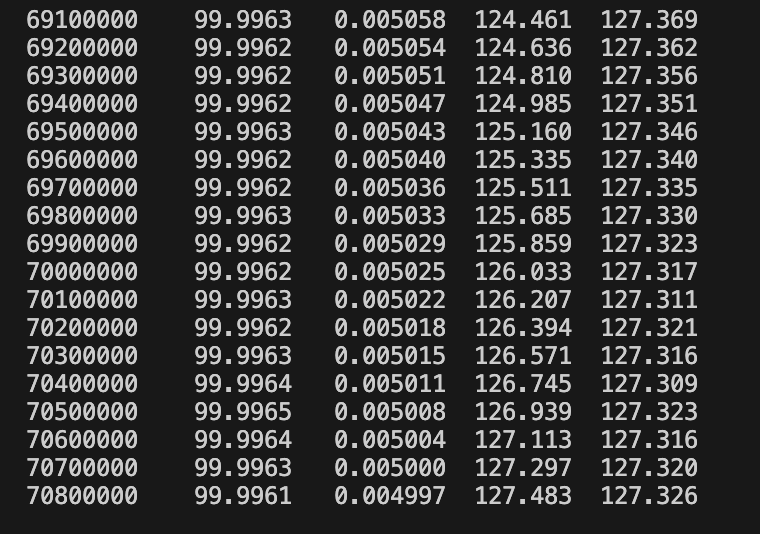
\includegraphics[width=0.8\textwidth]{Screenshot_1.png}
\end{figure}


\centerline{Screenshot of Output for Problem 2:}
\begin{figure}[H]
    \centering
    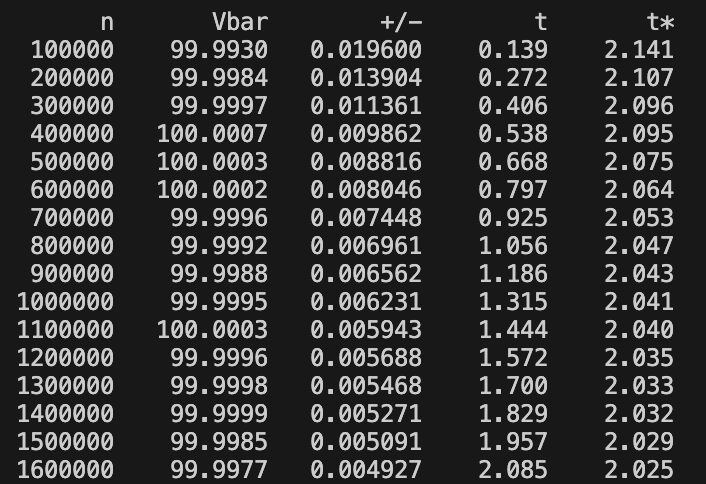
\includegraphics[width=0.8\textwidth]{Screenshot_2.png}
\end{figure}
\pagebreak

\centerline{Screenshot of Output for Problem 3:}
\begin{figure}[H]
    \centering
    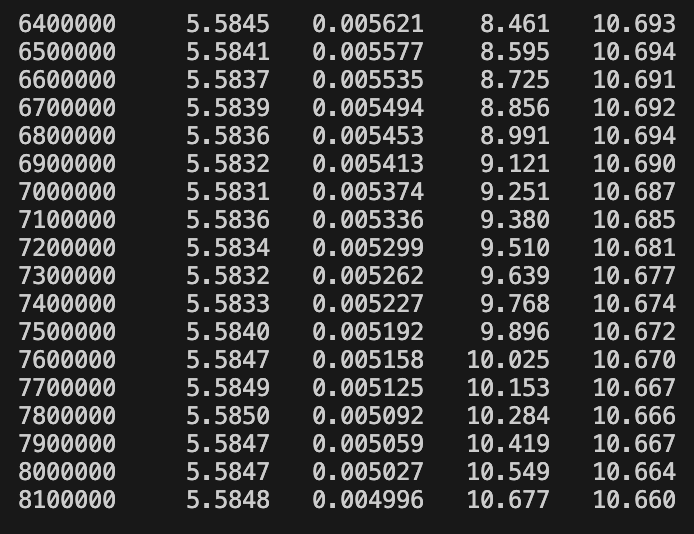
\includegraphics[width=0.8\textwidth]{Screenshot_3.png}
\end{figure}

\centerline{Screenshot of Output for Problem 4:}
\begin{figure}[H]
    \centering
    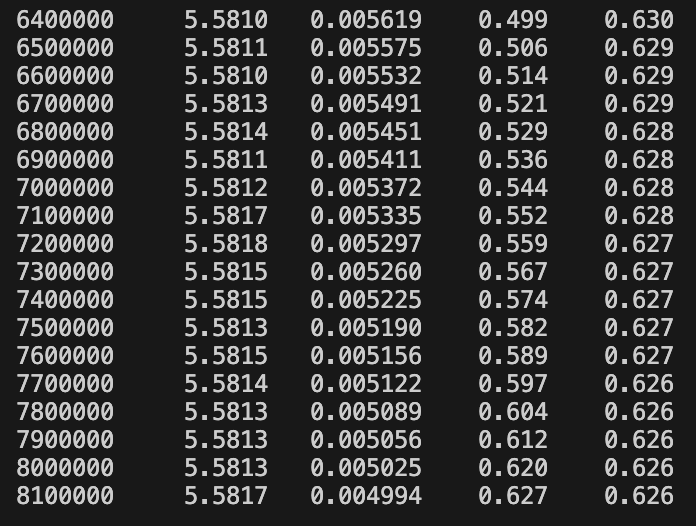
\includegraphics[width=0.8\textwidth]{Screenshot_4.png}
\end{figure}

\pagebreak

\centerline{Screenshot of Output for Problem 5:}
\begin{figure}[H]
    \centering
    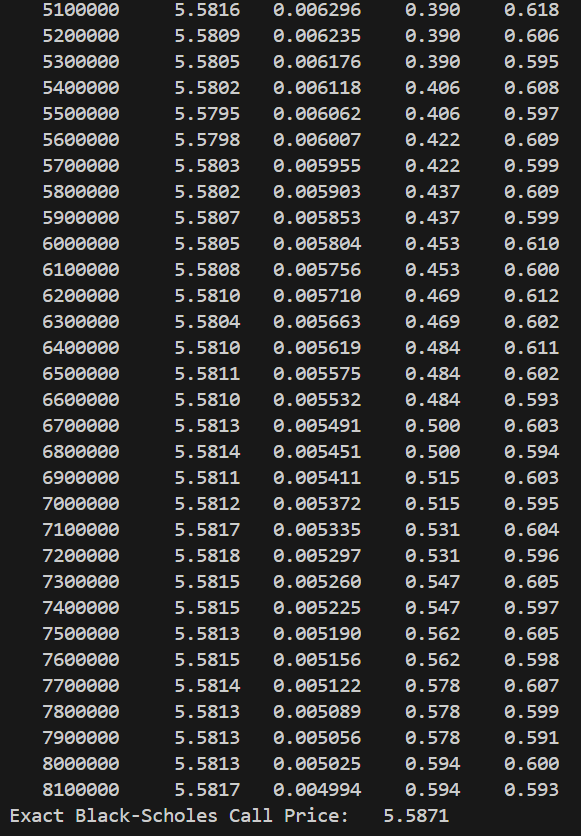
\includegraphics[width=0.8\textwidth]{Screenshot_5.png}
\end{figure}

\pagebreak

\centerline{Screenshot of Output for Problem 6:}
\begin{figure}[H]
    \centering
    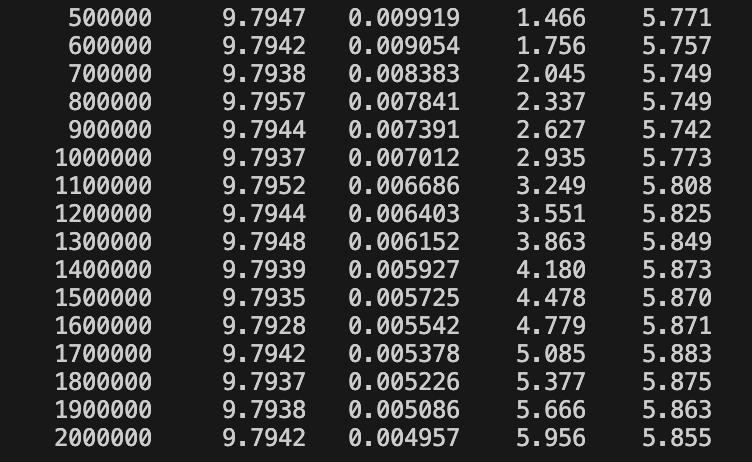
\includegraphics[width=0.8\textwidth]{Screenshot_6.png}
\end{figure}

\centerline{Screenshot of Output for Problem 7:}
\begin{figure}[H]
    \centering
    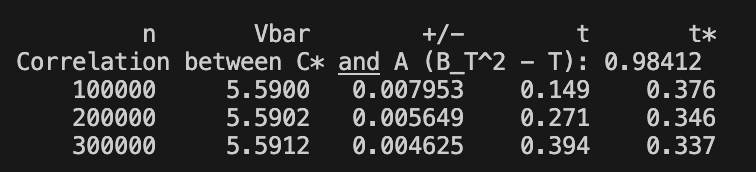
\includegraphics[width=0.8\textwidth]{Screenshot_7.png}
\end{figure}
\pagebreak

\centerline{Screenshot of Output for Problem 8:}
\begin{figure}[H]
    \centering
    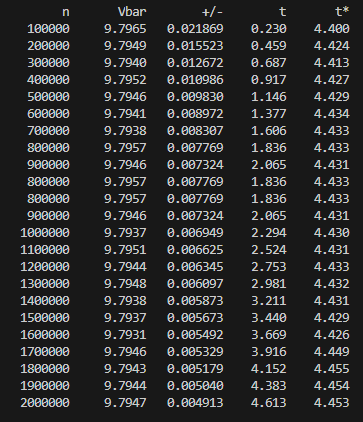
\includegraphics[width=0.8\textwidth]{Screenshot_8.png}
\end{figure}

\centerline{Screenshot of Output for Problem 9:}
\begin{figure}[H]
    \centering
    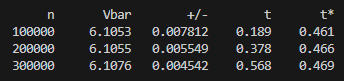
\includegraphics[width=0.8\textwidth]{Screenshot_9.png}
\end{figure}

\pagebreak
\subsection*{Code}
Code for Problem 2:
\begin{lstlisting}
#include "Functions.h"

int main() {
   double r, t, T, mu, sigma, dt, sqrtdt, S, S_anti, S0, V, Vbar, V2bar,
          elapsed_time, t_star, stdhatV, error, epsilon, n,
          U, Z, B, B_anti;
   int i, N, done, test;

   // Time to expiration.
   T = 0.5;

   // Number of stock price periods.
   N = 50;

   // Time increment per period.
   dt = T / N;

   // Compute this often-used value once and for all.
   sqrtdt = sqrt(dt);

   // Risk-free interest rate.
   r = 0.05;

   // Stock price volatility.
   sigma = .30;

   // Drift term.
   mu = r - sigma*sigma/2.0;

   // Initial stock price.
   S0 = 100.0;

   // Specify the 95% error tolerance.
   epsilon = 0.005;

   // Seed the RNG.
   MTUniform ();

   // Start the clock to time the computations.
   Time ();

   // Print column headings for output to execution window.
   printf ("         n       Vbar        +/-        t       t*\n");

   // Initialize certain values.
   V2bar = Vbar = done = n = test = 0;

   // Begin the simulation loop.
   while (!done) {
      // Initialize the stock price.
      S = S0;

      // Initialize the Brownian path.
      B = 0;
      B_anti = 0;

      // Initialize time.
      t = 0;

      // Simulate a stock price path.  Go forward period-by-period computing
      //   the next stock price.
      for (i = 1; i <= N; i++) {

         // Advance the path.
         U = MTUniform ();
         Z = PsiInv (U); // Standard normal via inverse transform.
         B += sqrtdt * Z; // Standard Brownian motion
         B_anti -= sqrtdt * Z; // Antithetic Brownian motion

         // Advance time by one period.
         t += dt;
      }
      // Compute the stock price at maturity using geometric Brownian motion
      S = S0 * exp (mu*t + sigma * B); // Standard path
      S_anti = S0 * exp(mu * t + sigma * B_anti); // Antithetic path

      // Discount back to time 0.
      V = exp(-r*T) * (S + S_anti) / 2; // Antithetic estimator

      // Update the simulation counter and the sample moments of V at time T.
      n ++;
      Vbar  = ((n-1)*Vbar + V) / n;
      V2bar = ((n-1)*V2bar + V*V) / n;

      // Update the error condition test counter.
      test ++;

      // Test the error condition periodically.
      if (test == 100000) {

         // Estimate the standard deviation of V.
         stdhatV  = sqrt (V2bar - Vbar*Vbar);

          // Estimate the error of the Vbar estimator.
         error = 1.96 * stdhatV / sqrt(n);

         // Compute the elapsed time and estimate the time of completion.
         elapsed_time = Time ();
         t_star = elapsed_time * pow (error / epsilon, 2);

         // Report.
         printf ("%10.0f   %8.4f   %8.6f %8.3f %8.3f\n", n, Vbar, error, elapsed_time, t_star);

         // Reset the "test" counter and see if error tolerance is met.
         test = 0;
         if (error < epsilon) {
            done = 1;
         }
      }
   }
   // Hold the window open until the user hits return.
   Exit ();
}
\end{lstlisting}
\pagebreak

Code for Problem 3:
\begin{lstlisting}
#include "Functions.h"

int main() {
   double r, t, T, mu, sigma, dt, sqrtdt, S, S_anti, S0, V, Vbar, V2bar,
          elapsed_time, t_star, stdhatV, error, epsilon, n, K,
          U, Z, B, B_anti;
   int i, N, done, test;

   // Time to expiration.
   T = 0.5;

   // Number of stock price periods.
   N = 50;

   // Time increment per period.
   dt = T / N;

   // Compute this often-used value once and for all.
   sqrtdt = sqrt(dt);

   // Risk-free interest rate.
   r = 0.05;

   // Stock price volatility.
   sigma = .30;

   // Drift term.
   mu = r - sigma * sigma / 2.0;

   // Initial stock price.
   S0 = 100.0;

   // Strike price for the European call option.
   K = 110.0;

   // Specify the 95% error tolerance.
   epsilon = 0.005;

   // Seed the RNG.
   MTUniform();

   // Start the clock to time the computations.
   Time();

   // Print column headings for output to execution window.
   printf("         n       Vbar        +/-        t       t*\n");

   // Initialize certain values.
   V2bar = Vbar = done = n = test = 0;

   // Begin the simulation loop.
   while (!done) {

      // Initialize the Brownian motion paths.
      B = 0;   
      B_anti = 0; 
      // Initialize time
      t = 0;

      // Simulate a stock price path. Move forward period-by-period computing
      //   the next stock price.
      for (i = 1; i <= N; i++) {

         // Generate a uniform random variable and transform it to standard normal.
         U = MTUniform();
         Z = PsiInv(U);  // Standard normal variable via inverse transform.

         // Advance the Brownian motion path.
         B += sqrtdt * Z; 
         B_anti -= sqrtdt * Z;

         // Advance time by one period.
         t += dt;
      }

      // Compute the stock price at maturity using geometric Brownian Motion.
      S = S0 * exp(mu * T + sigma * B); 
      S_anti = S0 * exp(mu * T + sigma * B_anti); 

      // Compute the call option payoff for both standard and antithetic paths.
      double C = fmax(S - K, 0);  
      double C_anti = fmax(S_anti - K, 0);

      // Compute the variance-reduced Monte Carlo estimator using Antithetic Variance Reduction
      double C_star = (C + C_anti) / 2; 

      // Discount back to time 0.
      V = exp(-r * T) * C_star;  // Expected discounted payoff

      // Update the simulation counter and the sample moments of V at time T.
      n++; 
      Vbar  = ((n-1) * Vbar + V) / n; 
      V2bar = ((n-1) * V2bar + V * V) / n; 

      // Update the error condition test counter.
      test++;

      // Test the error condition periodically.
      if (test == 100000) {

         // Estimate the standard deviation of V.
         stdhatV  = sqrt(V2bar - Vbar * Vbar);

         // Estimate the error of the Vbar estimator.
         error = 1.96 * stdhatV / sqrt(n);

         // Compute the elapsed time and estimate the time of completion.
         elapsed_time = Time();
         t_star = elapsed_time * pow(error / epsilon, 2);

         // Report.
         printf("%10.0f   %8.4f   %8.6f %8.3f %8.3f\n", n, Vbar, error, elapsed_time, t_star);

         // Reset the "test" counter and check if error tolerance is met.
         test = 0;
         if (error < epsilon) {
            done = 1;
         }
      }
   }

   // Hold the window open until the user hits return.
   Exit();
}
\end{lstlisting}

\pagebreak

Code for Problems 4 and 5:
\begin{lstlisting}
#include "Functions.h"

int main() {

   double r, T, mu, sigma, dt, sqrtdt, S, S_anti, S0, V, Vbar, V2bar,
          elapsed_time, t_star, stdhatV, error, epsilon, n, K,
          U, Z, Z_anti;
   int N, done, test;

   // Time to expiration.
   T = 0.5;

   // Number of stock price periods.
   N = 1;

   // Time increment per period
   dt = T / N;

   // Compute square root of dt.
   sqrtdt = sqrt(dt);

   // Risk-free interest rate.
   r = 0.05;

   // Stock price volatility.
   sigma = 0.30;

   // Drift term 
   mu = r - sigma * sigma / 2.0;

   // Initial stock price.
   S0 = 100.0;

   // Strike price for the European call option.
   K = 110.0;

   // Specify the 95% error tolerance.
   epsilon = 0.005;

   // Seed the RNG
   MTUniform();

   // Start the clock to time the computations.
   Time();

   // Print column headings for output to execution window.
   printf("         n       Vbar        +/-        t       t*\n");

   // Initialize certain values.
   V2bar = Vbar = done = n = test = 0;

   // Begin the simulation loop
   while (!done) {

      // Generate a uniform random variable and transform it to standard normal.
      U = MTUniform();
      Z = PsiInv(U); // Standard normal variable.
      Z_anti = -Z; // Antithetic counterpart.

      // Compute stock price at maturity using geometric Brownian Motion.
      S = S0 * exp(mu * T + sigma * sqrtdt * Z);
      S_anti = S0 * exp(mu * T + sigma * sqrtdt * Z_anti);

      // Compute the call option payoff for both standard and antithetic paths.
      double C = fmax(S - K, 0);
      double C_anti = fmax(S_anti - K, 0);

      // Compute the variance-reduced Monte Carlo estimator using Antithetic Variance Reduction.
      double C_star = (C + C_anti) / 2; 

      // Discount back to time 0.
      V = exp(-r * T) * C_star;  // Expected discounted payoff.

      // Update the simulation counter and the sample moments of V at time T.
      n++;
      Vbar  = ((n-1) * Vbar + V) / n;
      V2bar = ((n-1) * V2bar + V * V) / n;

      // Update the error condition test counter.
      test++;

      // Test the error condition periodically.
      if (test == 100000) {

         // Estimate the standard deviation of V.
         stdhatV  = sqrt(V2bar - Vbar * Vbar);

         // Estimate the error of the Vbar estimator.
         error = 1.96 * stdhatV / sqrt(n);

         // Compute the elapsed time and estimate the time of completion.
         elapsed_time = Time();
         t_star = elapsed_time * pow(error / epsilon, 2);

         // Report.
         printf("%10.0f   %8.4f   %8.6f %8.3f %8.3f\n", n, Vbar, error, elapsed_time, t_star);

         // Reset the "test" counter and check if error tolerance is met.
         test = 0;
         if (error < epsilon) {
            done = 1;
         }
      }
   }

   // Compute theoretical price of call option using Black Scholes formula
   double call_BS = BlackScholes(T, S0, K, sigma, r); 
   printf("Exact Black-Scholes Call Price: %8.4f\n", call_BS);

   // Hold the window open until the user hits return.
   Exit();
}
\end{lstlisting}

\pagebreak

Code for Problem 6:
\begin{lstlisting}
#include "Functions.h"

int main() {

   double r, t, T, mu, sigma, dt, sqrtdt, S, S_anti, S0, V, Vbar, V2bar,
          elapsed_time, t_star, stdhatV, error, epsilon, n, K,
          U, Z, B, B_anti, A, Abar, A2bar, Cbar, CAbar, C2bar, a_star;

   int i, N, done, test;

   // Time to expiration.
   T = 0.5;

   // Number of stock price periods.
   N = 50;  // Ensure full Brownian path

   // Time increment per period.
   dt = T / N;

   // Compute this often-used value once and for all.
   sqrtdt = sqrt(dt);

   // Risk-free interest rate.
   r = 0.05;

   // Stock price volatility.
   sigma = .30;

   // Drift term.
   mu = r - sigma*sigma/2.0;

   // Initial stock price.
   S0 = 100.0;

   // Strike price for the European call option.
   K = 110.0;

   // Specify the 95% error tolerance.
   epsilon = 0.005;

   // Seed the RNG.
   MTUniform();

   // Initial phase: Estimate Var A, Cov(X, A)
   Abar = A2bar = Cbar = CAbar = C2bar = 0;
   for (n = 1; n <= 5000; n++) {

      // Initialize Brownian motion paths
      B = 0;
      B_anti = 0;

      // Simulate a stock price path
      for (i = 1; i <= N; i++) {
         U = MTUniform();
         Z = PsiInv(U);
         B += sqrtdt * Z;
         B_anti -= sqrtdt * Z;
      }

      // Compute final stock prices
      S = S0 * exp(mu * T + sigma * B);
      S_anti = S0 * exp(mu * T + sigma * B_anti);

      // Compute option payoffs
      double C = fmax(S - K, 0);
      double C_anti = fmax(S_anti - K, 0);
      double C_star = (C + C_anti) / 2;

      // Define the new control variable
      A = B;

      // Update sample moments
      Abar  = ((n-1) * Abar + A) / n; // Mean of A
      A2bar = ((n-1) * A2bar + A * A) / n; // Mean of A^2
      Cbar  = ((n-1) * Cbar + C_star) / n; // Mean of C*
      C2bar = ((n-1) * C2bar + C_star * C_star) / n; // Mean of C*^2
      CAbar = ((n-1) * CAbar + C_star * A) / n; // Mean of C* * A
   }

   // Compute covariance and variance
   double cov_C_A = CAbar - Cbar * Abar;
   double var_A = A2bar - Abar * Abar;
   double var_C = C2bar - Cbar * Cbar;

   // Compute standard deviations
   double std_A = sqrt(var_A);
   double std_C = sqrt(var_C);

   // Compute correlation coefficient between C* and A
   double correlation = cov_C_A / (std_A * std_C);

   // Compute optimal a* for variance reduction
   a_star = -cov_C_A / var_A;

   // Print the correlation coefficient
   printf("Correlation between C* and A: %0.5f\n", correlation);

   // Start the clock to time the computations
   Time();

   // Print column headings for output to execution window.
   printf("\n");
   printf("         n       Vbar        +/-        t       t*\n");

   // Initialize certain values
   Vbar = V2bar = n = done = test = 0;
   
   // Begin the simulation loop
   while (!done) {

      // Initialize Brownian motion paths
      B = 0;
      B_anti = 0;

      // Simulate a stock price path
      for (i = 1; i <= N; i++) {
         U = MTUniform();
         Z = PsiInv(U);
         B += sqrtdt * Z;
         B_anti -= sqrtdt * Z;
      }

      // Compute the stock price at maturity using geometric Brownian motion
      S = S0 * exp(mu * T + sigma * B);
      S_anti = S0 * exp(mu * T + sigma * B_anti);

      // Compute option payoffs
      double C = fmax(S - K, 0);
      double C_anti = fmax(S_anti - K, 0);
      double C_star = (C + C_anti) / 2;

      // Compute the new control variable
      A = B;

      // Discount back to time 0 using control variable adjustment
      V = exp(-r * T) * (C_star + a_star * A);

      // Update sample moments
      n++;
      Vbar  = ((n-1) * Vbar + V) / n;
      V2bar = ((n-1) * V2bar + V * V) / n;

      // Update the error condition test counter.
      test++;

      // Test the error condition periodically.
      if (test == 100000) {

         // Estimate the standard deviation of V.
         stdhatV  = sqrt(V2bar - Vbar*Vbar);

         // Estimate the error of the Vbar estimator.
         error = 1.96 * stdhatV / sqrt(n);

         // Compute the elapsed time and estimate the time of completion.
         elapsed_time = Time();
         t_star = elapsed_time * pow(error / epsilon, 2);

         // Report.
         printf ("%10.0f   %8.4f   %8.6f %8.3f %8.3f\n", n, Vbar, error, elapsed_time, t_star);

         // Reset the "test" counter and check if error tolerance is met.
         test = 0;
         if (error < epsilon) {
            done = 1;
         }
      }
   }

   // Hold the window open until the user hits return.
   Exit();
}
\end{lstlisting}
\pagebreak

Code for Problem 7:
\begin{lstlisting}
#include "Functions.h"

int main() {

   double r, t, T, mu, sigma, dt, sqrtdt, S, S_anti, S0, V, Vbar, V2bar,
          elapsed_time, t_star, stdhatV, error, epsilon, n, K,
          U, Z, B, B_anti, A, Abar, A2bar, Cbar, CAbar, C2bar, a_star;

   int i, N, done, test;

   // Time to expiration.
   T = 0.5;

   // Number of stock price periods.
   N = 50;  // Ensure full Brownian path

   // Time increment per period.
   dt = T / N;

   // Compute this often-used value once and for all.
   sqrtdt = sqrt(dt);

   // Risk-free interest rate.
   r = 0.05;

   // Stock price volatility.
   sigma = .30;

   // Drift term.
   mu = r - sigma*sigma/2.0;

   // Initial stock price.
   S0 = 100.0;

   // Strike price for the European call option.
   K = 110.0;

   // Specify the 95% error tolerance.
   epsilon = 0.005;

   // Seed the RNG.
   MTUniform();

   // Initial phase: Estimate Var A, Cov(X, A)
   Abar = A2bar = Cbar = CAbar = C2bar = 0;
   for (n = 1; n <= 5000; n++) {

      // Initialize Brownian motion paths
      B = 0;
      B_anti = 0;

      // Simulate a stock price path
      for (i = 1; i <= N; i++) {
         U = MTUniform();
         Z = PsiInv(U);
         B += sqrtdt * Z;
         B_anti -= sqrtdt * Z;
      }

      // Compute final stock prices
      S = S0 * exp(mu * T + sigma * B);
      S_anti = S0 * exp(mu * T + sigma * B_anti);

      // Compute option payoffs
      double C = fmax(S - K, 0);
      double C_anti = fmax(S_anti - K, 0);
      double C_star = (C + C_anti) / 2;

      // Define the new control variable
      A = B * B - T;

      // Update sample moments
      Abar  = ((n-1) * Abar + A) / n; // Mean of A
      A2bar = ((n-1) * A2bar + A * A) / n; // Mean of A^2
      Cbar  = ((n-1) * Cbar + C_star) / n; // Mean of C*
      C2bar = ((n-1) * C2bar + C_star * C_star) / n; // Mean of C*^2
      CAbar = ((n-1) * CAbar + C_star * A) / n; // Mean of C* * A
   }

   // Compute covariance and variance
   double cov_C_A = CAbar - Cbar * Abar;
   double var_A = A2bar - Abar * Abar;
   double var_C = C2bar - Cbar * Cbar;

   // Compute standard deviations
   double std_A = sqrt(var_A);
   double std_C = sqrt(var_C);

   // Compute correlation coefficient between C* and A
   double correlation = cov_C_A / (std_A * std_C);

   // Compute optimal a* for variance reduction
   a_star = -cov_C_A / var_A;

   // Print the correlation coefficient
   printf("Correlation between C* and A: %0.5f\n", correlation);

   // Start the clock to time the computations
   Time();

   // Print column headings for output to execution window.
   printf("\n");
   printf("         n       Vbar        +/-        t       t*\n");

   // Initialize certain values
   Vbar = V2bar = n = done = test = 0;
   
   // Begin the simulation loop
   while (!done) {

      // Initialize Brownian motion paths
      B = 0;
      B_anti = 0;

      // Simulate a stock price path
      for (i = 1; i <= N; i++) {
         U = MTUniform();
         Z = PsiInv(U);
         B += sqrtdt * Z;
         B_anti -= sqrtdt * Z;
      }

      // Compute the stock price at maturity using geometric Brownian motion
      S = S0 * exp(mu * T + sigma * B);
      S_anti = S0 * exp(mu * T + sigma * B_anti);

      // Compute option payoffs
      double C = fmax(S - K, 0);
      double C_anti = fmax(S_anti - K, 0);
      double C_star = (C + C_anti) / 2;

      // Compute the new control variable
      A = B * B - T;

      // Discount back to time 0 using control variable adjustment
      V = exp(-r * T) * (C_star + a_star * A);

      // Update sample moments
      n++;
      Vbar  = ((n-1) * Vbar + V) / n;
      V2bar = ((n-1) * V2bar + V * V) / n;

      // Update the error condition test counter.
      test++;

      // Test the error condition periodically.
      if (test == 100000) {

         // Estimate the standard deviation of V.
         stdhatV  = sqrt(V2bar - Vbar*Vbar);

         // Estimate the error of the Vbar estimator.
         error = 1.96 * stdhatV / sqrt(n);

         // Compute the elapsed time and estimate the time of completion.
         elapsed_time = Time();
         t_star = elapsed_time * pow(error / epsilon, 2);

         // Report.
         printf ("%10.0f   %8.4f   %8.6f %8.3f %8.3f\n", n, Vbar, error, elapsed_time, t_star);

         // Reset the "test" counter and check if error tolerance is met.
         test = 0;
         if (error < epsilon) {
            done = 1;
         }
      }
   }

   // Hold the window open until the user hits return.
   Exit();
}
}
\end{lstlisting}

\pagebreak

Code for Problem 8:
\begin{lstlisting}
#include "Functions.h"

int main() {

   double r, t, T, mu, sigma, dt, sqrtdt, S, S_anti, S0, V, Vbar, V2bar,
          elapsed_time, t_star, stdhatV, error, epsilon, n, K,
          U, Z, B, B_anti, A, Abar, A2bar, Cbar, CAbar, C2bar, a_star,
          S_max, S_anti_max;  // Track the max stock prices along each path


   int i, N, done, test;
   // Time to expiration.
   T = 0.5;

   // Number of stock price periods.
   N = 50;

   // Time increment per period.
   dt = T / N;

   // Compute this often-used value once and for all.
   sqrtdt = sqrt(dt);

   // Risk-free interest rate.
   r = 0.05;

   // Stock price volatility.
   sigma = .30;

   // Drift term.
   mu = r - sigma * sigma / 2.0;

   // Initial stock price.
   S0 = 100.0;

   // Strike price for the European call option.
   K = 110.0;

   // Specify the 95% error tolerance.
   epsilon = 0.005;

   // Seed the RNG.
   MTUniform();

   // Initial phase: Estimate Var A, Cov(X, A)
   Abar = A2bar = Cbar = CAbar = C2bar = 0;
   for (n = 1; n <= 5000; n++) {

      // Initialize Brownian motion paths
      B = 0;
      B_anti = 0;

      // Initialize stock price and max stock price trackers
      S = S0;
      S_anti = S0;
      S_max = S0;
      S_anti_max = S0;

      // Simulate a stock price path and track the max price
      for (i = 1; i <= N; i++) {
         U = MTUniform();
         Z = PsiInv(U);
         B += sqrtdt * Z;
         B_anti -= sqrtdt * Z;
         
         S = S0 * exp(mu * (i * dt) + sigma * B);
         S_anti = S0 * exp(mu * (i * dt) + sigma * B_anti);

         // Update max values encountered so far in the path
         if (S > S_max) S_max = S;  
         if (S_anti > S_anti_max) S_anti_max = S_anti;
      }

      // Compute the look-back option payoff 
      double L = fmax(S_max - K, 0);
      double L_anti = fmax(S_anti_max - K, 0);
      double C_star = (L + L_anti) / 2;  // Antithetic variance reduction applied

      // Define the new control variable
      A = B * B - T;

      // Update sample moments
      Abar  = ((n-1) * Abar + A) / n;
      A2bar = ((n-1) * A2bar + A * A) / n;
      Cbar  = ((n-1) * Cbar + C_star) / n;
      C2bar = ((n-1) * C2bar + C_star * C_star) / n;
      CAbar = ((n-1) * CAbar + C_star * A) / n;
   }

   // Compute covariance and variance for control variate adjustment
   double cov_C_A = CAbar - Cbar * Abar;
   double var_A = A2bar - Abar * Abar;
   double var_C = C2bar - Cbar * Cbar;

   // Compute standard deviations
   double std_A = sqrt(var_A);
   double std_C = sqrt(var_C);

   // Compute correlation coefficient
   double correlation = cov_C_A / (std_A * std_C);

   // Compute optimal a*
   a_star = -cov_C_A / var_A;

   // Print the correlation coefficient
   printf("Correlation between C* and A (B_T^2 - T): %0.5f\n", correlation);

   // Start the clock to time the computations
   Time();

   // Print column headings for output to execution window.
   printf("\n");
   printf("         n       Vbar        +/-        t       t*\n");

   // Initialize certain values
   Vbar = V2bar = n = done = test = 0;

   // Begin the simulation loop
   while (!done) {

      // Initialize Brownian motion paths
      B = 0;
      B_anti = 0;

      // Initialize stock price and max stock price trackers
      S = S0;
      S_anti = S0;
      S_max = S0;
      S_anti_max = S0;

      // Simulate a stock price path and track the max price
      for (i = 1; i <= N; i++) {
         U = MTUniform();
         Z = PsiInv(U);
         B += sqrtdt * Z;
         B_anti -= sqrtdt * Z;

         S = S0 * exp(mu * (i * dt) + sigma * B);
         S_anti = S0 * exp(mu * (i * dt) + sigma * B_anti);

         // Update max values encountered so far in the path
         if (S > S_max) S_max = S;  
         if (S_anti > S_anti_max) S_anti_max = S_anti;
      }

      // Compute the look-back option payoff (depends on max stock price)
      double L = fmax(S_max - K, 0);
      double L_anti = fmax(S_anti_max - K, 0);
      double C_star = (L + L_anti) / 2;  // Antithetic variance reduction applied

      // Compute the new control variable
      A = B * B - T;

      // Discount back to time 0 using control variable adjustment
      V = exp(-r * T) * (C_star + a_star * A);

      // Update sample moments
      n++;
      Vbar  = ((n-1) * Vbar + V) / n;
      V2bar = ((n-1) * V2bar + V * V) / n;

      // Update the error condition test counter
      test++;

      // Test the error condition periodically.
      if (test == 100000) {
         
         // Estimate the standard deviation of V.
         stdhatV  = sqrt(V2bar - Vbar * Vbar);

         // Estimate the error of the Vbar estimator.
         error = 1.96 * stdhatV / sqrt(n);
         
         // Compute the elapsed time and estimate the time of completion.
         elapsed_time = Time();
         t_star = elapsed_time * pow(error / epsilon, 2);
         
         // Report.
         printf ("%10.0f   %8.4f   %8.6f %8.3f %8.3f\n", n, Vbar, error, elapsed_time, t_star);
        
         // Reset the "test" counter and check if error tolerance is met.
         test = 0;
         if (error < epsilon) {
            done = 1;
         }
      }
   }

   // Hold the window open until the user hits return.
   Exit();
}


\end{lstlisting}

\pagebreak
Code for Problem 9:

\begin{lstlisting}
#include "Functions.h"

int main() {

   double r, t, T, mu, sigma, dt, sqrtdt, S, S_anti, S0, V, Vbar, V2bar,
          elapsed_time, t_star, stdhatV, error, epsilon, n, K,
          U, Z, B, B_anti, A, Abar, A2bar, Cbar, CAbar, C2bar, a_star,
          S_tau, S_anti_tau;
    
    int i, N, done, test;

   // Time to expiration.
   T = 0.5;

   // Number of stock price periods.
   N = 50;

   // Time increment per period.
   dt = T / N;

   // Compute this often-used value once and for all.
   sqrtdt = sqrt(dt);

   // Risk-free interest rate.
   r = 0.05;

   // Stock price volatility.
   sigma = .30;

   // Drift term.
   mu = r - sigma * sigma / 2.0;

   // Initial stock price.
   S0 = 100.0;

   // Strike price for the European call option.
   K = 110.0;

   // Specify the 95% error tolerance.
   epsilon = 0.005;

   // Seed the RNG.
   MTUniform();

   // Initial phase: Compute Var A, Cov(X, A)
   Abar = A2bar = Cbar = CAbar = C2bar = 0;
   for (n = 1; n <= 5000; n++) {

      // Initialize Brownian motion paths
      B = 0;
      B_anti = 0;
      S = S0;
      S_anti = S0;
      S_tau = S0; // Store shouted price for standard path
      S_anti_tau = S0; // Store shouted price for antithetic path
      bool shouted = false; // Track whether shout has been triggered
      bool shouted_anti = false;

      // Simulate a stock price path and track the max price
      for (i = 1; i <= N; i++) {
         U = MTUniform();
         Z = PsiInv(U);
         B += sqrtdt * Z;
         B_anti -= sqrtdt * Z;

         S = S0 * exp(mu * (i * dt) + sigma * B);
         S_anti = S0 * exp(mu * (i * dt) + sigma * B_anti);
        
         // Shouting Strategy: Lock in price as soon as S_t > K
         if (!shouted && S > K) {
             S_tau = S;
             shouted = true;
         }
         if (!shouted_anti && S_anti > K) {
             S_anti_tau = S_anti;
             shouted_anti = true;
         }
      }

      // Compute shout option payoff: max(S_T - K, S_tau - K, 0)
      double C_shout = fmax(fmax(S - K, S_tau - K), 0);
      double C_shout_anti = fmax(fmax(S_anti - K, S_anti_tau - K), 0);
      double C_star = (C_shout + C_shout_anti) / 2;

      // Define the control variable
      A = B * B - T;

      // Update sample moments
      Abar  = ((n-1) * Abar + A) / n;
      A2bar = ((n-1) * A2bar + A * A) / n;
      Cbar  = ((n-1) * Cbar + C_star) / n;
      C2bar = ((n-1) * C2bar + C_star * C_star) / n;
      CAbar = ((n-1) * CAbar + C_star * A) / n;
   }

   // Compute covariance and variance
   double cov_C_A = CAbar - Cbar * Abar;
   double var_A = A2bar - Abar * Abar;
   double var_C = C2bar - Cbar * Cbar;

   // Compute standard deviations
   double std_A = sqrt(var_A);
   double std_C = sqrt(var_C);

   // Compute correlation coefficient
   double correlation = cov_C_A / (std_A * std_C);

   // Compute optimal a*
   a_star = -cov_C_A / var_A;

   // Print the correlation coefficient
   printf("Correlation between C* and A (B_T^2 - T): %0.5f\n", correlation);

   // Start the clock to time the computations
   Time();

   // Print column headings for output to execution window.
   printf("\n");
   printf("         n       Vbar        +/-        t       t*\n");

   // Initialize certain values
   Vbar = V2bar = n = done = test = 0;

   while (!done) {

      B = 0;
      B_anti = 0;
      S = S0;
      S_anti = S0;
      S_tau = S0;
      S_anti_tau = S0;
      bool shouted = false;
      bool shouted_anti = false;
    
      // Simulate stock path
      for (i = 1; i <= N; i++) {
         U = MTUniform();
         Z = PsiInv(U);
         B += sqrtdt * Z;
         B_anti -= sqrtdt * Z;

         S = S0 * exp(mu * (i * dt) + sigma * B);
         S_anti = S0 * exp(mu * (i * dt) + sigma * B_anti);


         // **Shouting Strategy: Shout as soon as S_t > K**
         if (!shouted && S > K) {
             S_tau = S;
             shouted = true;
         }
         if (!shouted_anti && S_anti > K) {
             S_anti_tau = S_anti;
             shouted_anti = true;
         }
      }

      // Compute the shout option payoff (depends on shouted price and stock price at maturity)
      double C_shout = fmax(fmax(S - K, S_tau - K), 0);
      double C_shout_anti = fmax(fmax(S_anti - K, S_anti_tau - K), 0);
      double C_star = (C_shout + C_shout_anti) / 2;

      // Compute the new control variable
      A = B * B - T;

      // Discount back to time 0 using control variable adjustment
      V = exp(-r * T) * (C_star + a_star * A);

      // Update sample moments
      n++;
      Vbar  = ((n-1) * Vbar + V) / n;
      V2bar = ((n-1) * V2bar + V * V) / n;

      // Update the error condition test counter
      test++;

      if (test == 100000) {
         // Estimate the standard deviation of V.
         stdhatV = sqrt(fmax(0, V2bar - Vbar * Vbar));

         // Estimate the error of the Vbar estimator.
         error = 1.96 * stdhatV / sqrt(n);

         // Compute the elapsed time and estimate the time of completion.
         elapsed_time = Time();
         t_star = elapsed_time * pow(error / epsilon, 2);

         // Report.
         printf ("%10.0f   %8.4f   %8.6f %8.3f %8.3f\n", n, Vbar, error, elapsed_time, t_star);
        
         // Reset the "test" counter and see if error tolerance is met.
         test = 0;
         if (error < epsilon) {
            done = 1;
         }
      }
   }
   // Hold the window open until the user hits return.
   Exit();
}

\end{lstlisting}
\end{document}
